Так же в третьей главе рассматривается параметрический метод оценки частоты на основе авторегрессионной (АР) - модели сигнала.

Удобство применения АР для задачи оценки частоты обусловлено тем, что в сигнале с расширенным спектром после демодуляции ПСП остается одна
гармоническая компонента и шум (\ref{eq:cdma_strip_eq}).  Даже если входной сигнал содержал другие гармонические компоненты,
после повторной модуляции они будут "размазаны" по спектру.

Для обнаружения одного гармонического сигнала на фоне аддитивной помехи в виде белого шума достаточно использовать АР модель второго порядка.

Но на качество оценки параметра сильное значение имеет качетво оценки АКФ. Для оценки, удовлетворяющий начальной расстройке частоты,
необходима более точная оценка АКФ, чем можно получить вычисляя АКФ без предварительно компенсации шума.

Компенсация шума с помощью предлагаемого итеративного алгоритма позволяет достичь заданной точности при уровне ОСШ -25 дБ, в то
время как без компенсации шума заданная точность может быть достигнута только при уровне 10 дБ - рисунок \ref{pic:ACF_boost}.

\begin{figure}[H]
\center\scalebox{1}{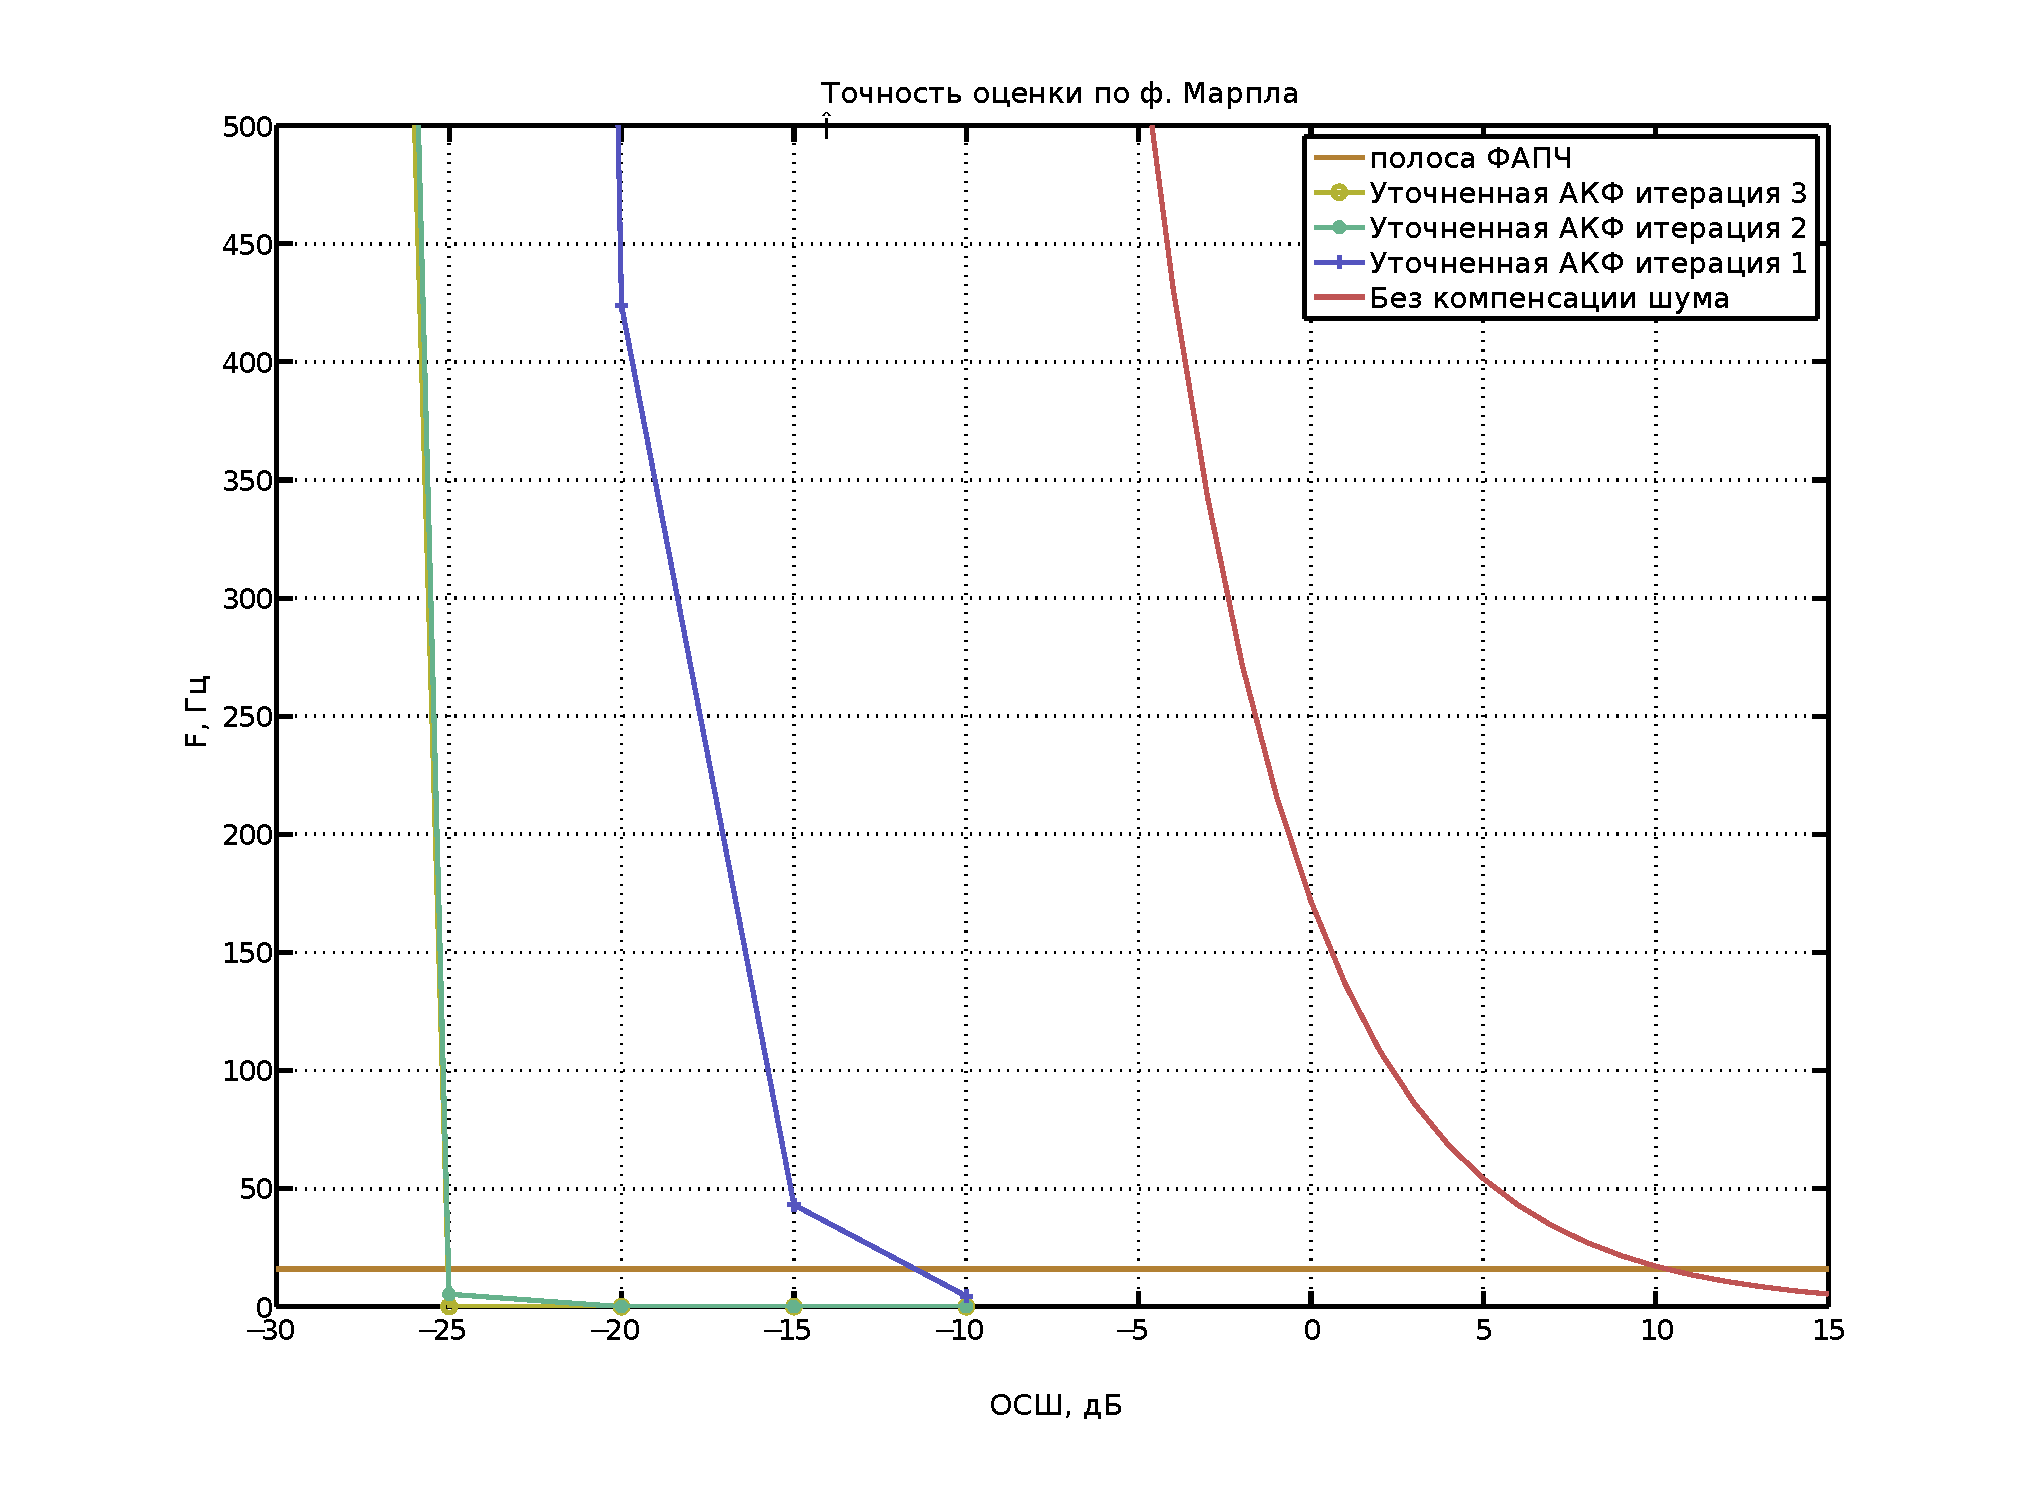
\includegraphics[width=1\linewidth]{ACF_boost.eps}}
	\caption{Точность оценки частоты с компенсацией и без компенсации шума}
	\label{pic:ACF_boost}
\end{figure}
